\subsection{How a query cracks a multi-dimensional partial index}
\label{subsec:mcrack}

%n-columns\\
%n-predicates*\\


%\subsection{Section To Do...}
%\label{subsec:todo}
%\textcolor{red}{There are many critical issues that we have to address in this section.
%Here is an order of their presentation.
%\begin{enumerate}
%\item What do we store in a kd-tree in adaptive clustering -> Each node stores a k-dimensional query and the first position of the ``right'' partition (split position). Define properly the k-dimensional queries.
%\item How do we insert nodes in the kd-tree.
%\item During insertion of a node(->cracking action) we need to know the limits of the to-be-cracked partition. How do we decide the limits while traversing the tree?
%\item How do we decide which partitions will be scanned/cracked/included/omitted in order to get the final row ids of the tuples that qualify the predicate.
%\item How can the kd-tree be used to answer different queries on the same dimensions (or a subset of the dimensions).
%\end{enumerate}}
%\textcolor{red}{We should also examine whether a $kd$-tree can be used for a subset of $k$ columns or not. Ideally, the same $kd$-tree should be used for any subset of the $k$ columns, where the creation of the tree was based on. For instance, if the $kd$-tree is built based on queries on $\{\mathtt{C_1,C_3,C_5,C_6}\}$, then the same $kd$-tree can be used to qualify queries just on $\{\mathtt{C_3,C_5}\}$}.

In this section we describe in detail the steps we follow to answer a multi-dimensional query $\mathtt{Q^k}$.
To answer such a query with sideways cracking, we would need $\mathtt{k-1}$ cracker maps.
The head of all cracker maps would be the same attribute.
Thus, we would need to replicate the head attribute $\mathtt{k-1}$ times.
All cracker maps are reorganized based on the head, i.e., cracking the head and reorganize the tail at the same time, to ensure alignment.
The cracker index and the cracker tape is updated with the new cracking steps on the head of the cracker maps.
In order to find the qualifying tuples of each attribute, we need to scan those tuples that qualify the head predicate and create an intermediate bit vector for every cracker map.
In the end we need to apply a conjunction on all intermediate bit vectors to retrieve the final qualifying tuples out of a contiguous piece in memory.

\begin{figure}[t]
\begin{center}
\vspace*{3\baselineskip}
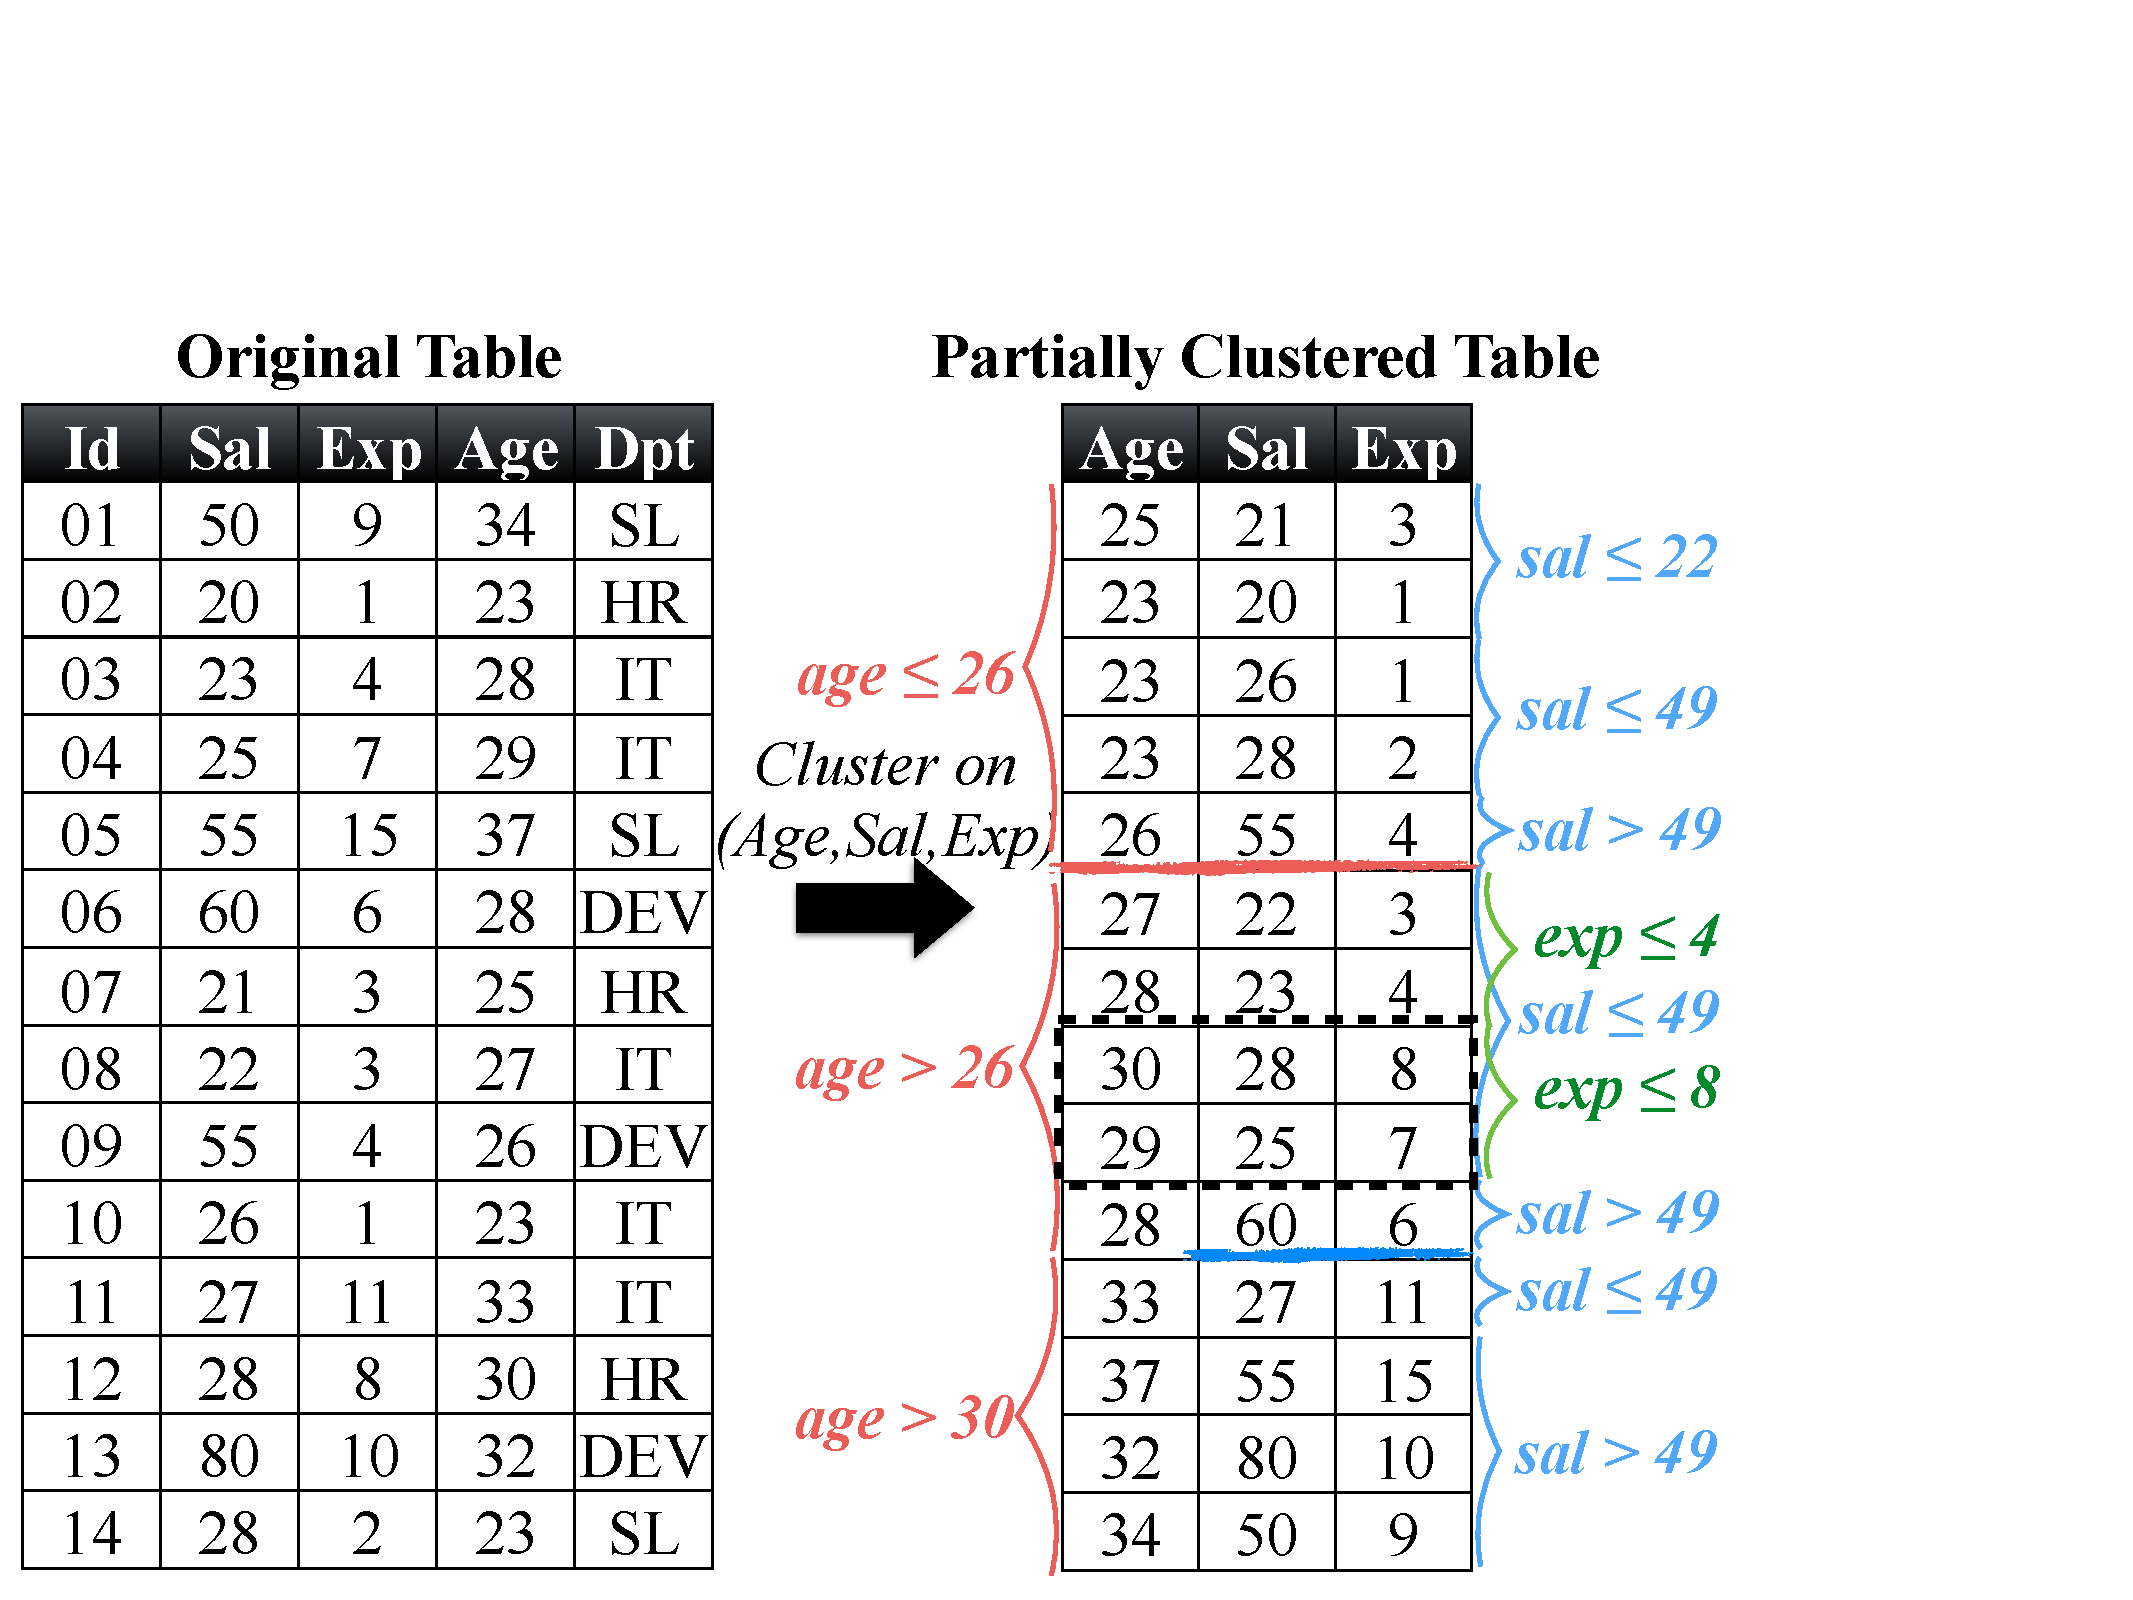
\includegraphics[trim=0cm 2cm 0cm 8.5cm, width=\columnwidth]{Figures/mcrack_relation_full}
\caption{Multidimensional search on partially clustered data.}
\label{fig:mcluster_full}
\end{center}
\end{figure}

To avoid copying the head $\mathtt{k-1}$ times, we could have a cracker map that includes of all $\mathtt{k}$ attributes.
A brute-force approach would be to reorganize every column based on all respective predicates for every query and maintain this information in a proper index.
Figure~\ref{fig:mcluster_full} shows an example.
All resulting tuples lay in a contiguous area in memory (the dashed box), which we can immediately return without extra bit vector operations.
However, with this approach, for every query $\mathtt{Q^k}$ we need to create at most $\mathtt{3^k}$ partitions after cracking $\mathtt{k}$ attributes.
To store the information for each partition we need a tree-structure similar to a quad-tree, but with $\mathtt{3^k}$ child nodes per parent node.
It is obvious that with such an approach we would hit very fast \emph{the curse of dimensionality} wall.

A solution between sideways cracking which cracks only one dimension and cracking all dimensions based on all attributes as we described in the previous paragraph, seems to be the trade-off we are looking for.
In our approach, we suggest to create a cracker map consisting of $\mathtt{k}$ attributes, i.e., a cluster map.
For every query, we crack at most two of the $\mathtt{k}$ attributes.
Which attributes to crack and how is automatically given from the index structure we use.
We explain in the next section how the index defines the cracking attributes.

Figure~\ref{fig:pcluster} shows an example of a query with range predicates on three attributes, e.g., Q1.
To answer this query we first crack column $\mathtt{Age}$ and then column $\mathtt{Salary}$ on one of the two predicates included in every range.
After cracking the two columns, we have a list of candidate tuples which we need to scan in order to find tuples that qualify for all predicates.
To produce the final result, we can use a conjunction between intermediate bit vectors, since the columns are aligned.

To reduce data access for future queries, we can navigate to clusters with candidate qualifying tuples by using a cracker index.
In the next section we describe our index structure and its vital role not only on maintaining information about the partitions but also deciding which attributes to crack and how for every query.
